\documentclass{standalone}
\usepackage{pgfplots}
\usepackage{amsmath}
\usepackage{textcomp}
\pgfplotsset{compat=1.18}

\begin{document}

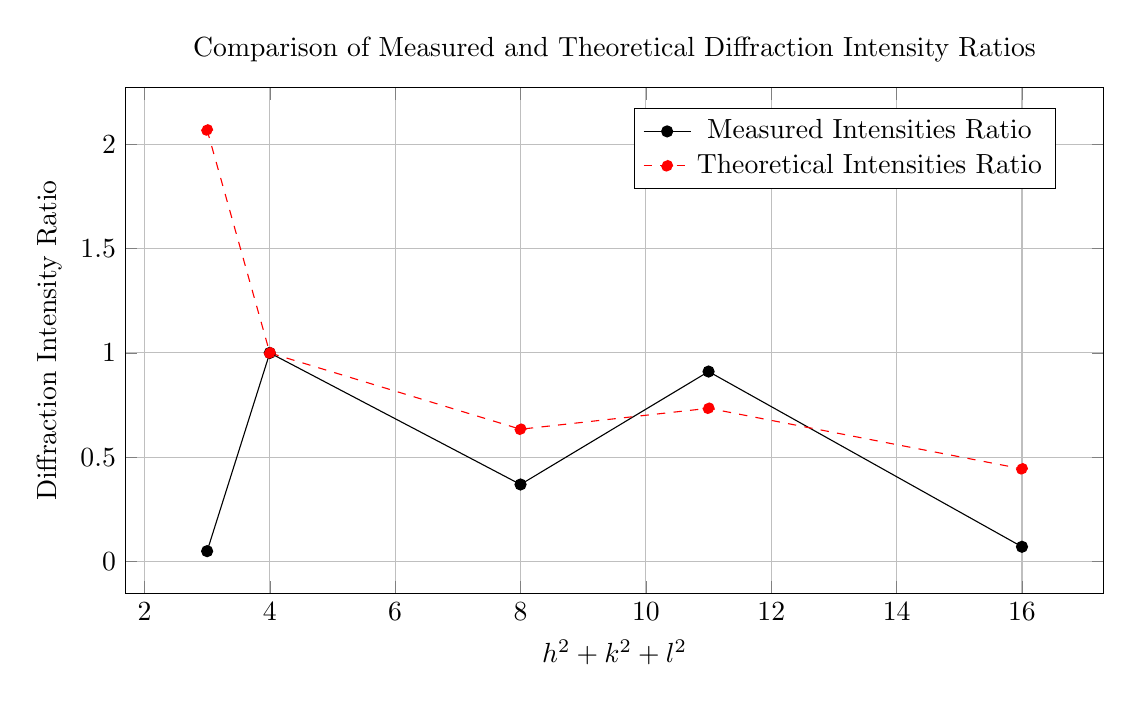
\begin{tikzpicture}
\begin{axis}[
    xlabel={$h^2 + k^2 + l^2$},
    ylabel={Diffraction Intensity Ratio},
    title={Comparison of Measured and Theoretical Diffraction Intensity Ratios},
    grid=both,
    width=14cm,
    height=8cm,
    legend style={at={(0.52,0.96)}, anchor=north west}
]

% 実験データ点
\addplot[
    mark=*,
    color=black,
]
coordinates {
  (3,0.050828)
  (4,1)
  (8,0.370026)
  (11,0.91082)
  (16,0.071749)
};
\addlegendentry{Measured Intensities Ratio}
\addplot[
    mark=*,
    color=red,
    dashed,
]
coordinates {
  (3,2.067503)
  (4,1)
  (8,0.634527)
  (11,0.735008)
  (16,0.444863)
};
\addlegendentry{Theoretical Intensities Ratio}
\end{axis}
\end{tikzpicture}

\end{document}